% !TeX encoding = utf8
% !TeX spellcheck = en_GB

\section{Minimize Heat Exposure}

We are presenting a two-step approach to supported people to reduce their heat stress in their everyday life. First we are presenting an approach to find a route for pedestrian with a minimal heat exposure. On this basis, we show an approach to find a point in time with a minimal heat exposure, for instance to go shopping in a supermarket.

\subsection{Finding a Route with Minimal Heat Exposure \label{sec:optimal-route}}

\subsubsection{Modelling as a Time-Dependent Routing Problem}

Finding a route with minimal heat exposure can be modelled as time-dependent routing problem, where the edge weighting function is not static and instead may vary over time. Subsequently, many speed up techniques developed for static routing problems like bi-directional search cannot simply be applied \parencite{Delling2009}. 

Below, we are representing the road network as undirected graph $G=(V,E,w_d,w_h)$, where $V$ is the set of vertices or nodes (e.g. junctions) and $E\subseteq V\times V$ is the set of edges (e.g. road segments) each connecting a pair of nodes. Furthermore $w_d: E \to \mathbb{R}_{\geq 0}$ and $w_h: E \times T \to \mathbb{R}_{\geq 0}$ are to edge weighting function, at which:
\begin{itemize}
	\item $w_d(e)$ is the length of the edge $e$, and
	\item $w_h(e, t)$ is the heat exposure of edge $e$ at time $t$.
\end{itemize}   
Hereafter, a path $p$ from node $v_0$ to node $v_k$ starting a time $t_0$ is denoted as sequence of edge-time pairs $((e_{v_0v_1},t_0),(e_{v_1v_2},t_1),\dots, (e_{v_{k-1}v_k},t_{k-1}))$, where $t_i$ is the time at which node $v_i$ is leaved. The weight of an edge is fixed at the time the traversing of the edge is started \parencite[the so-called frozen link model,][]{Orda1990}. The time $t_i$ can be computed as follows: $t_i := t_{i-1} + t_{walk}(e_{v_{i-1},v_i})$ where $t_{walk}(e_{v_{i-1},v_i})$ is the time needed by a pedestrian to traverse the edge $e_{v_{i-1},v_i}$. The starting time $t_0$ is ether given or set to~$0$. 

To compute the weight of a path $w_h(p)$ the following formula can be applied:
	\begin{equation}\label{eq:path-weight}
		w_h(p) := \sum_{(e,t) \in p} w_h(e, t).
	\end{equation}
Those means we are looking for the path $p^*$ from a node $v$ to a node $u$ that has the minimal weight of all possible path from $v$ to $u$. Below, we are using $w_h(p, t)$ to denote the weight of the path $p$ starting at time $t$. 

The time-dependent routing problem is $\mathcal{NP}$-hard, if it is not allowed to wait on a node and the FIFO (first in, first out) property is not fulfilled \parencite{Orda1990}. A~weighting function $w$ fulfils the FIFO property if the change of the edge weight decreases not faster than the change in the actual time $t$ increases \parencite{Kaufman1993}. 

Usually, we cannot assume that $w_h$ fulfils the FIFO property, because the function most of the time depends on the air temperature and, in general the air temperature can decrease more than actual time increases. Since, most people are not willing to wait at a node as well, finding a route with a minimal heat exposure is $\mathcal{NP}$-hard.
Therefore, hereafter the edge weighting is frozen at the starting time $t_0$ so that we have static route planning problem and classic algorithms like  \citeauthor{Dijkstra1959}'s algorithm \parencite{Dijkstra1959} can be applied. 

\subsubsection{The Edge Weighting Function \label{sec:edge-weighting}}

\begin{figure}
	\centering
	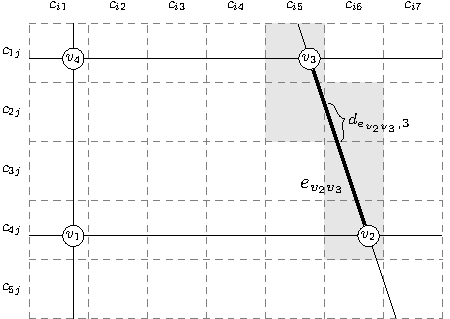
\includegraphics{figures/raster-edge-mapping-standalone}
	\caption[Example for the raster to edge mapping]{An 
		example for the raster to edge mapping.}
	\label{fig:raster-edge-mapping}
\end{figure}

To find a route with a minimal heat exposure it is key to define the edge weighting function in an appropriated way. At this, it is not sufficient to only take the actual thermal comfort in to account, we also must consider the time a person is exposed to heat. Below, we assume that the time of exposure is proportional to the length of the edge $w_d$ \parencite[following][]{Hasenfratz2015}. Based on this assumption we are defining the edge weighting function $w_h$ as follows: 
\begin{equation}\label{eq:edge-weight}
w_h(e, t) := \sum_{c \in Intersec(e)} d_c \cdot h_c(t).
\end{equation}
Here, the thermal comfort values (like air temperature or heat index) are represented as time-dependent raster $H(t) = \left(h_{ij}(t)\right)$, where $h_{ij}(t)$ denotes the thermal comfort value in raster cell $c_{ij}$ at time $t \in T$. In the formula above, $Intersec(e)$ is the set of raster cells intersected by the edge $e$ and $d_c$ the length of the intersection of $e$ with raster cell $c$.  That is, to obtain the edge weight, the value of each intersected raster cell is weighted with the length of the intersection and then accumulated, as shown in figure~\ref{fig:raster-edge-mapping}.

Using the actual thermal comfort measures -- air temperature and heat index -- we get the following edge weighting functions:
\begin{align}
	\label{eq:edge-weight-temperature}
	w_{T_a}(e,t)& = \sum_{c \in Intersec(e)} d_c \cdot T_a(t, c),
\end{align}
for the air temperature and respectively:
\begin{align}
	\label{eq:edge-weight-heatindex}
	w_{HI}(e,t)& = \sum_{c \in Intersec(e)} d_c \cdot T_{HI}\left(T_a(t, c), RH(t)\right)
\end{align}
for the heat index. Here, $T_a(t,c)$ is the air temperature in raster cell $c$ at time $t \in T$, $RH(t)$ is the relative humidity at time $t$ and $T_{HI}$ is Steadman's heat index. How we obtained those values is described below in section \ref{sec:data-sets}.

 \subsection{Finding the Optimal Time \label{sec:find-optimal-time}}
 
 Apart from selecting a route with minimal heat exposure the risk of heat stress in the everyday life (e.g. go shopping in a supermarket) can massively be reduced by selecting the appropriate time for this action. That's because usually, the heat exposure is highest at middays and significant lower in the morning or evening.
 
 To give recommendations for a time with minimal heat exposure, we use a three step procedure: 
 
 \begin{enumerate}
 	\item \label{itm:nearby-search} Perform a nearby search originating from a given starting point $s$  (e.g. address or GPS coordinates) to find all locations $L$ that fulfils a certain search criteria (e.g. is supermarket or pharmacy)  within a specified radius $r$ (e.g. \SI{500}{\meter}).
 	
 	\item \label{itm:optimal-time} For each location $\ell \in L$ found in step \ref{itm:nearby-search}, determine the point in time $t^*$ with the lowest heat exposure. 
 	
 	\item \label{itm:ranking} Create a ranking of the locations in $L$ based on the minimum heat exposure found in step \ref{itm:optimal-time}, so that the location with the lowest heat exposure has rank 1.
 \end{enumerate} 

The steps \ref{itm:nearby-search} and \ref{itm:ranking} are not very complicated, so we are focusing on step \ref{itm:optimal-time}. 

\subsubsection{Modelling as a Optimization Problem} 

By finding the time with the lowest heat exposure for a location $\ell \in L$. we should consider certain constrains like the opening hours $[t_{open}(\ell),t_{close}(\ell)]$ of $\ell$. As the objective function to minimize we are using the heat exposure of the optimal path between the starting point $s$ and location $\ell$, as proposed above in section \ref{sec:optimal-route}. Those, finding the time with the minimal heat exposure means to minimize the following objective function $h(\ell, t)$:
	\begin{equation}\label{eq:objective-funtion}
		h(\ell, t) = w_h(p^*, t) = \min_{p\in P_{s\ell}} w_h(p, t) = \min_{p\in P_{s\ell}} \sum_{(e, t') \in p} w_h(e, t'),
	\end{equation}
where $P_{s\ell}$ is the set of all possible paths from $s$ to $\ell$,  $w_h(p, t)$ is the accumulated edge weight of all edges in $p$ at starting time $t$ and $w_h$ is the edge weighting function from equation \eqref{eq:edge-weight}. 

Using the objective function defined in equation \eqref{eq:objective-funtion}, we can formulate the problem to find a time with minimal heat exposure as a optimization problem with constrains:
\begin{subequations}
	\label{eq:optimal-time}
	\begin{alignat}{2}
	&\min_{t \in T} h(\ell, t) && \label{eq:optimal-time:of} \\
	%& \text{s.t.} &  t_{open}(\ell)  \leq t &\leq t_{close}(\ell) \label{eq:optimal-time:oh} \\
	&\text{s.t.} & t & \geq t_{open}(\ell)-t_{walk}(\ell, t) \label{eq:optimal-time:twm}\\
	&	& t & \leq   t_{close}(\ell)-(t_{walk}(\ell, t)+t_{buff}(\ell))	\label{eq:optimal-time:twe}\\
	&	&  t & \geq t_{earliest} \label{eq:optimal-time:te} \\
	&	&  t & \leq t_{latest} \label{eq:optimal-time:tl} \\
	&  & t  & \geq t_{now} \label{eq:optimal-time:tn} 
	\end{alignat}
\end{subequations}

Note, that the location $\ell$ is fixed, as the selection of the location with lowest heat exposure is performed later in step \ref{itm:ranking}. The constrains \eqref{eq:optimal-time:twm} and \eqref{eq:optimal-time:twe} are  basically ensuring that the location is arrived within the opening hours. We must ensure that the shop can be reached before it closes, therefore we have to consider the time needed to walk to the location $\ell$ ($t_{walk}(\ell)$) as well as the time needed to perform e.g. the purchase ($t_{buff}(\ell)$). On the other hand, it can make sense to start early in the morning to arrive the location $\ell$ just in time when its opening, so we are subtracting the walking time from the opening time. The constrains \eqref{eq:optimal-time:te} and \eqref{eq:optimal-time:tl} are an earliest respectively latest time desired by the user and can be omitted. Finally, the last constrain  \eqref{eq:optimal-time:tn}  guarantees, that the optimal time is in the future. Another thing to notice is, that the walking time $t_{walk}(\ell, t)$ depends on the starting time $t$, because conditional on the time a different (properly longer) optimal route can be selected.

 \subsubsection{Optimization \label{sec:optimization}}
 
 To find the optimal time, we need a optimization method without derivatives, because the objective function $h(\ell, t)$ is not necessarily derivable. One such method is Brent's method \parencite{Brent2002}, a procedure for the approximation of local optima within an interval $[x_1, x_2]$.
 
 In order to apply Brent's method, we have to transform the constrains \eqref{eq:optimal-time:twm}-\eqref{eq:optimal-time:tn} to a lower and upper limit of an interval.  The constrains \eqref{eq:optimal-time:twm}, \eqref{eq:optimal-time:te} and \eqref{eq:optimal-time:tn} can  be easily converted to a lower limit, as follows: 
  	\begin{equation}\label{eq:lower-limit}
  		t_{lower}(\ell, t) = \max\left\lbrace  t_{open}(\ell)-t_{walk}(\ell, t), t_{now}, t_{earliest} \right\rbrace.
  	\end{equation}
  Alike, we can transform the constrains \eqref{eq:optimal-time:twe} and \eqref{eq:optimal-time:tl} to an upper limit:
  	\begin{equation}\label{eq:upper-limit}
  		t_{upper}(\ell, t) = \min\left\lbrace  t_{close}(\ell)- (t_{walk}(\ell, t) + t_{buff}(\ell)), t_{latest} \right\rbrace.
  	\end{equation}
 It's simple to recognize, that the interval $[t_{lower}(\ell, t), t_{upper}(\ell, t)]$ preserves the constrains from the optimization problem defined above in equation \eqref{eq:optimal-time}.  
 
 However, Brent's method can still not be applied, since -- as outlined above in section \ref{sec:optimization} -- the lower and upper limit of the interval is depending on the starting time $t$ and therefore, not static as required for Brent's method. As solution to avoid this problem we are proposing the introduction of a penalty term:
 \begin{equation}
 \label{eq:optimal-time-penality}
 h'(t,\ell) = \begin{cases}
 h(t,\ell) & \text{if }t \in [t_{lower}(\ell, t), t_{upper}(\ell, t)],\\
 h(t,\ell)  + c & \text{otherwise,}
 \end{cases}
 \end{equation}
 where $c$ is a large constant such that $h(t,\ell) + c$ is never selected as optimal solution, if the constrains are violated. Now, we can use the walking time $t_{walk}^{shortest}(\ell)$  for the shortest route for the lower and upper limit. Finally, we can formulate the optimization problem for Brent's method as follows:
 \begin{subequations}
 	\label{eq:brent-optimization-problem}
 	\begin{alignat}{2}
 	&\min_{t \in T} h'\ell, t) && \\
 	&\text{s.t.} & t & \geq \max\left\lbrace  t_{open}(\ell)-t_{walk}^{shortest}(\ell), t_{now}, t_{earliest} \right\rbrace \\
 	& & t &\leq \min\left\lbrace  t_{close}(\ell)- \left(t_{walk}^{shortest}(\ell) + t_{buff}(\ell)\right), t_{latest} \right\rbrace.
 	\end{alignat}
 \end{subequations}
Now we can use Brent's method to find for each location $\ell$ the optimal time $t^*$. To avoid, that the Brent optimizer is trapped in a local optimum, it can be executed several times with different random start points.
